\subsection{Éléments d'identification du \emph{Particle Flow}}\label{chapter-LHC-section-evt_reco-subsec-PF_elements}
\subsubsection{Traces des particules chargées et vertex}\label{chapter-LHC-section-evt_reco-subsec-PF_elements-subsubsec-tracks}
\paragraph{Traces des particules chargées}
Les particules chargées laissent des traces de leur passage dans le trajectographe et, dans le cas des muons, dans les chambres à muons.
Le trajectographe, présenté section~\ref{chapter-LHC-section-CMS-subsec-tracker}, ne donne pas de traces continues mais des points de passage de ces particules.
\par
Les traces des particules sont reconstruites à partir de ces points de passage à l'aide d'une méthode itérative~\cite{particle-flow,track_reco}.
Un détecteur de traces par combinaison basé sur un filtre de Kalman (KF) \cite{Kalman_filter} reconstruit les traces selon la procédure suivante:
\begin{enumerate}
\item Une trajectoire initiale est générée à partir d'un ajustement à quelques points de passages.
Cette trajectoire doit être compatible avec celle d'une particule chargée.
\item L'ensemble des points de passage devant correspondre à cette trajectoire est déterminé.
Ces points sont obtenus en extrapolant la trajectoire à travers le trajectographe.
À chaque ajout d'un point de passage, l'ajustement de la trajectoire à l'ensemble des points lui étant associés est mis à jour.
\item Une fois que l'ensemble des points pouvant être associés à la trajectoire ont été trouvés, un ajustement final est réalisé.
Il permet de déterminer l'ajustement optimal de la trajectoire aux points de passage.
Les propriétés de la particule chargée (origine, impulsion transverse, direction) sont ainsi déterminées.
La trace est acceptée ou rejetée selon des critères portant sur les paramètres de l'ajustement final.
Les points de passage associés à une trace acceptée sont retirés de la liste des points à traiter.
\end{enumerate}
Cette procédure est alors répétée en utilisant des critères de plus en plus précis afin d'augmenter l'efficacité de la reconstruction des traces.
Le taux de mauvaise reconstruction est quant à lui réduit en appliquant des critères de qualité sur les traces reconstruites.
%Plus de détails sont disponibles dans la référence~\cite{particle-flow}.
\subparagraph{Cas des électrons}
La reconstruction des électrons de haute énergie et isolés vis-à-vis des autres particules est naturellement basée sur les données du ECAL~\cite{electron_reco_8tev}.
La position et la valeur du dépôt d'énergie sont utilisés afin de déterminer les points de passage attendus dans le trajectographe pour l'électron (ou le positron).
Cependant, à cause de l'épaisseur du trajectographe, les électrons émettent avant de parvenir au ECAL une fraction de leur énergie par \emph{bremsstrahlung}, \ie\ sous forme de photons.
Les performances de reconstruction des électrons dépendent ainsi fortement de la capacité à identifier ces photons et mesurer leurs énergies.
Les dépôts d'énergie dans le ECAL (\emph{clusters}) dus à l'électron et aux photons potentiellement issus du \emph{bremsstrahlung} sont regroupés en un \emph{supercluster}.
Le \emph{supercluster} est construit à partir des dépôts du ECAL se situant dans une fenêtre fine en $\eta$ et plus large en $\phi$ afin de prendre en compte la courbure de la trajectoire de l'électron due au champ magnétique.
\par
Dans le cas des électrons contenus dans les jets, en revanche, un biais apparaît à cause des autres particules du jet situées à proximité de l'électron.
Cet effet mène à un fort taux de mauvaise reconstruction.
L'identification des électrons à partir du ECAL est ainsi limitée aux cas d'électrons isolés des autres particules.
Afin de reconstruire les électrons exclus par cette limitation, une approche basée sur les données du trajectographe a été développée~\cite{particle-flow}.
Dès qu'une trace reconstruite selon la procédure exposée précédemment vérifie $\pT>\SI{2}{\GeV}$, elle est considérée comme candidat électron.
\par
Lorsque l'électron émet peu d'énergie par \emph{bremsstrahlung}, l'ajustement de la trace correspondante est de bonne qualité à travers l'ensemble du trajectographe.
De plus, l'extrapolation de cette trace jusqu'à la surface du ECAL permet de lui faire correspondre un dépôt d'énergie.
L'énergie contenue dans le dépôt doit alors être compatible avec celle déterminée à partir de la trace.
\par
Plus l'électron émet de l'énergie par \emph{bremsstrahlung}, moins l'ajustement de la trace correspondante est de qualité, car cet ajustement ne prend pas en compte la perte d'énergie au cours de la propagation de l'électron.
Les traces correspondant à cette situation sont sélectionnées à partir du nombre de points de passage associés et du $\chi^2$ de l'ajustement.
Elles sont réajustées à partir d'un filtre de somme de gaussiennes (GSF, \emph{Gaussian Sum Filter}) \cite{GSF} utilisant cinq paramètres, plus adapté que le KF pour ces électrons~\cite{particle-flow}.
Un critère d'identification basé sur un arbre de décision (BDT, \emph{Boosted Decision Tree}) est appliqué sur cet ajustement, il est détaillé dans la section~\ref{chapter-LHC-section-evt_reco-subsec-ptc_ID}.
\subparagraph{Cas des muons}
%Les chambres à muons permettent d'identifier ces particules avec une grande efficacité.
%Les calorimètres, situés entre le point de collision et les chambres à muons, absorbent toutes les autres particules (à l'exception des neutrinos qui n'interagissent pas), permettant d'obtenir une bonne pureté quant aux particules se propageant dans les chambres à muons.
Les muons laissent des signaux de leur passage dans le trajectographe et dans les chambres à muons.
Trois types de muons peuvent être définis:
\begin{itemize}
\item les muons seuls (\emph{standalone muons}), reconstruits uniquement à partir des signaux des chambres à muons;
\item les muons globaux (\emph{global muons}), obtenus par la correspondance d'une trace dans le trajectographe avec l'extrapolation de la trace d'un muon seul;
\item les muons du trajectographe (\emph{tracker muons}) sont les traces du trajectographe d'impulsion transverse supérieure à \SI{0.5}{\GeV} dont l'extrapolation passe par une des chambres à muons ayant détecté le passage d'une particule.
\end{itemize}
\par
Lorsque des hadrons chargés arrivent au HCAL, ils se désintègrent en une gerbe hadronique.
Si des éléments de cette gerbe parviennent à traverser le HCAL (\emph{punch-through}), ils donnent un signal dans les chambres à muons.
Des critères d'identification sont alors appliqués aux traces afin de réduire les muons reconstruits à partir de hadrons.
Ils sont abordés dans la section~\ref{chapter-LHC-section-evt_reco-subsec-ptc_ID}.
\paragraph{Interactions avec le matériau du trajectographe}
Des interactions entre les particules issues des collisions et le matériau du trajectographe peuvent mener
à une déviation (\emph{kink})~\cite{moliere_scat_1,moliere_scat_2}
voire
à la production de vertex secondaires~\cite{particle-flow,CMS-TRK-17-001},
comme illustré sur la figure~\ref{fig-chapter-LHC-section-evt_reco-subsec-PF_elements-CMS-self-radio}.
Un algorithme a été développé~\cite{CMS-PAS-TRK-10-003} afin d'identifier les traces de particules ayant interagit avec le matériau du trajectographe.
\begin{figure}[h]
\centering
\subcaptionbox{Dans le plan longitudinal \plane{r}{z}.\label{subfig-chapter-LHC-section-evt_reco-subsec-PF_elements-particle-flow-Figure_005-a}}[.45\textwidth]
{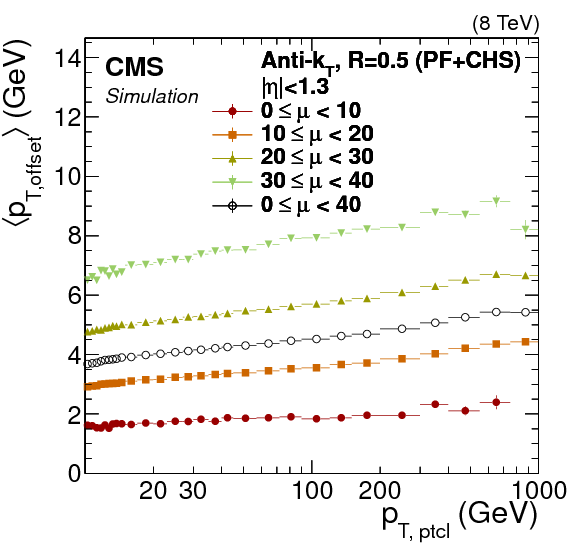
\includegraphics[width=.45\textwidth]{\PhDthesisdir/plots_and_images/from_particle-flow/Figure_005-a.png}}
\hfill
\subcaptionbox{Dans le plan transverse \plane{x}{y}.\label{subfig-chapter-LHC-section-evt_reco-subsec-PF_elements-particle-flow-Figure_005-b}}[.45\textwidth]
{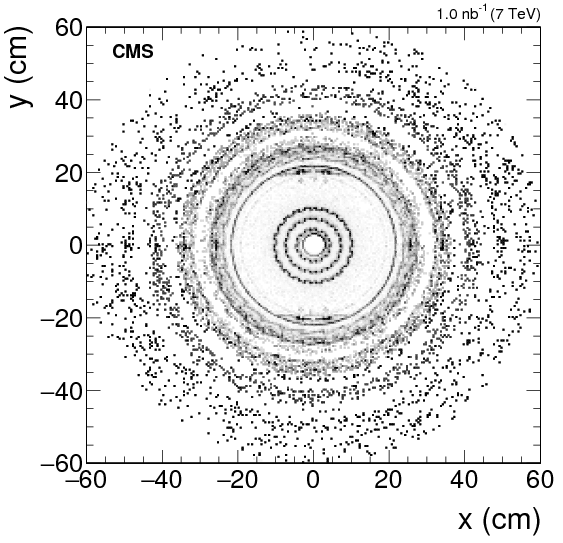
\includegraphics[width=.45\textwidth]{\PhDthesisdir/plots_and_images/from_particle-flow/Figure_005-b.png}}
\caption[Points d'interactions entre particules des événements et matière du détecteur.]{Carte des points d'interactions entre particules des événements et matière composant le détecteur~\cite{particle-flow,CMS-TRK-17-001} à partir de données prises en 2011 à $\sqrt{s}=\SI{7}{\TeV}$.}
\label{fig-chapter-LHC-section-evt_reco-subsec-PF_elements-CMS-self-radio}
\end{figure}
\paragraph{Vertex}
La combinaison des traces permet de reconstruire les vertex d'interactions de l'événement.
Plusieurs vertex sont présents du fait de l'empilement.
Le vertex principal est choisi comme étant le vertex dont la somme des impulsions transverses au carré des traces en provenant est la plus élevée, les autres sont considérés comme des vertex de l'empilement.
L'efficacité de reconstruction du vertex principal est ainsi de l'ordre de \SI{100}{\%}, celle des vertex de l'empilement de \SI{70}{\%}~\cite{JERC_RunI}.
\subsubsection{Dépôts dans les calorimètres}
\paragraph{Agglomération}
L'énergie d'une particule unique se répartit dans plusieurs cellules des calorimètres.
Les dépôts dans chacunes des cellules sont alors regroupés de proche en proche en agglomérats (\emph{clusters})~\cite{particle-flow}.
%Plusieurs raisons existent à cette agglomération:
%\begin{itemize}
%\item détecter et mesurer les énergies et directions des particules neutres stables comme les photons et les hadrons neutres;
%\item séparer ces particules neutres des particules chargées;
%\item reconstruire et identifier les électrons et les photons issus du \emph{bremsstrahlung} correspondant;
%\item améliorer la mesure de l'énergie des hadrons chargés dont les traces sont imprécises.
%\end{itemize}
\par La construction de ces agglomérats commence par l'identification des cellules des calorimètres mesurant une énergie supérieure à un seuil donné, défini pour chaque sous-partie des calorimètres.
Les seuils sont fixés à partir d'une optimisation sur des simulations de photons, \pionnull, \Kaonnull\ et jets.
Les cellules adjacentes sont ajoutées à l'agglomérat.
Puis, toute cellule avec au moins un coin en commun avec une cellule déjà dans l'agglomérat et mesurant une énergie supérieure à deux fois le niveau moyen du bruit est ajoutée à l'agglomérat.
%\par
%Afin d'identifier les photons issus du \emph{bremsstrahlung} d'un électron, les dépôts dans le ECAL pouvant correspondre à l'électron et à ces éventuels photons sont regroupés en un \emph{supercluster}.
%Le \emph{supercluster} est ainsi l'ensemble des \emph{clusters} dans le ECAL se situant à proximité de la direction de l'électron~\cite{particle-flow}.
\paragraph{Calibration}
Les photons et les hadrons neutres sont reconstruits à l'aide de leurs dépôts dans les calorimètres.
Des dépôts isolés vis-à-vis des traces de particules chargées sont une signature claire des particules neutres.
Cependant, un dépôt de particule neutre situé au même endroit qu'un dépôt de particule chargée ne peut être détecté que comme étant un excès d'énergie pour la particule chargée par rapport à l'énergie déterminée à l'aide du trajectographe.
Une bonne calibration de la réponse des calorimètres aux photons et aux hadrons est donc cruciale pour la bonne reconstruction des particules neutres.
Cette calibration a été réalisé dans un premier temps avant les premières collisions à l'aide de faisceaux de test.
Une fois les collisions commencées, les données issues des celles-ci sont exploitées afin de calibrer plus finement les calorimètres.
%Plus de détails sont disponibles dans la section~3.5 de la référence~\cite{particle-flow}.